\documentclass[tikz]{standalone}
\usetikzlibrary{intersections}
\begin{document}
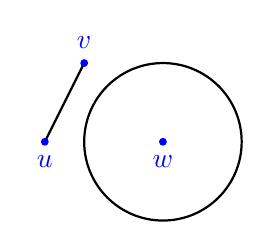
\begin{tikzpicture}
    \coordinate (u) at (1.5,0);
    \coordinate (v) at (2,1);
    \coordinate (w) at (3,0);

    \draw[thick] (u) -- (v);
    \draw[thick] (w) circle (1);

    \node[circle,fill,color=blue,inner sep=1pt,label={[text=blue]-90:\(u\)}] at (u) [] {}; 
    \node[circle,fill,color=blue,inner sep=1pt,label={[text=blue, above]:\(v\)}] at (v) [] {}; 
    \node[circle,fill,color=blue,inner sep=1pt,label={[text=blue]-90:\(w\)}] at (w) [] {}; 
\end{tikzpicture}
\end{document}
